\chapter{Calcul Littéral}\label{ChCalculLitteral}

\vspace{5cm}
\begin{acquis}
\begin{itemize}
\item simplifier une expression littérale en enlevant certains signes $\times$;
\item calculer une expression littérale pour une valeur particulière de la ou les inconnues;
\item écrire l'expression littérale correspondant à un problème simple.
\end{itemize}
\end{acquis}

\activites

\begin{activite}[Un carré sans coins]

\begin{minipage}[c]{0.28\linewidth}
 
\includegraphics[width=2.5cm]{parties_carre}
 \end{minipage} \hfill
 \begin{minipage}[c]{0.68\linewidth}
On a représenté ci-contre deux parties d'un carré. Il est constitué de petites cases ayant pour côté un carreau. Celles qui se trouvent sur les bords sont coloriées en rose, sauf les quatre coins.
  \end{minipage} \\

\begin{partie}
Réalise une figure de 3 carreaux de côté. Indique le nombre de cases roses. Recommence avec un carré de 4 carreaux de côté puis avec un carré de 5 carreaux de côté.
\end{partie}

\begin{partie}
Quel est le nombre de cases roses pour un carré de 6 carreaux de côté ? Et pour 12 carreaux ? Et pour 100 ?
\end{partie}

\begin{partie}
Le professeur appelle $x$ le nombre de carreaux d'un côté du carré et $G$ le nombre de cases roses. Des élèves ont obtenu les expressions suivantes : \\[0.4em]
\begin{center}
 \begin{tabularx}{0.9\linewidth}{X|X|X}
  Anis : $G = x \cdot 4 - 2$ & Chloé : $G = 4 \cdot (x - 2)$ & Enzo : $G = 4 \cdot x - 8$ \\
  Basile : $G = x - 2 \cdot 4$ & Dalila : $G = (x - 2) \cdot 4$ & Florian : $G = 4 \cdot x - 4$ \\
  \end{tabularx}   
 \end{center}
 \vspace{0.3cm}
Parmi ces expressions, lesquelles sont fausses ? Pourquoi ? Y a-t-il plusieurs bonnes réponses ? Justifie.
\end{partie}

\begin{partie}
Calcule le nombre de cases roses lorsque $x = 6$ puis $x = 24$ et enfin pour $x = 100$.
\end{partie}

\end{activite}


%%%%%%%%%%%%%%%%%%%%%%%%%%%%%%%%%%%
%%%%%%%%%%%%%%%%%%%%%%%%%%%%%%%%%%%
%MiseEnPage
%%%%%%%%%%%%%%%%%%%%%%%%%%%%%%%%%%%
\newpage
%%%%%%%%%%%%%%%%%%%%%%%%%%%%%%%%%%%
%%%%%%%%%%%%%%%%%%%%%%%%%%%%%%%%%%%

%%%%%%%%%%%%%%%%%%%%%%%%%%%%%%%%%%%%%%%%%%%%%%%%%%%%%%%%%%%%%%%%%%%%%%%

\begin{activite}[Rectangles cousins]

\begin{partie}
Calcule le périmètre et l'aire des deux rectangles suivants. Que remarques-tu ?

\begin{minipage}[c]{0.48\linewidth}
 \begin{center} 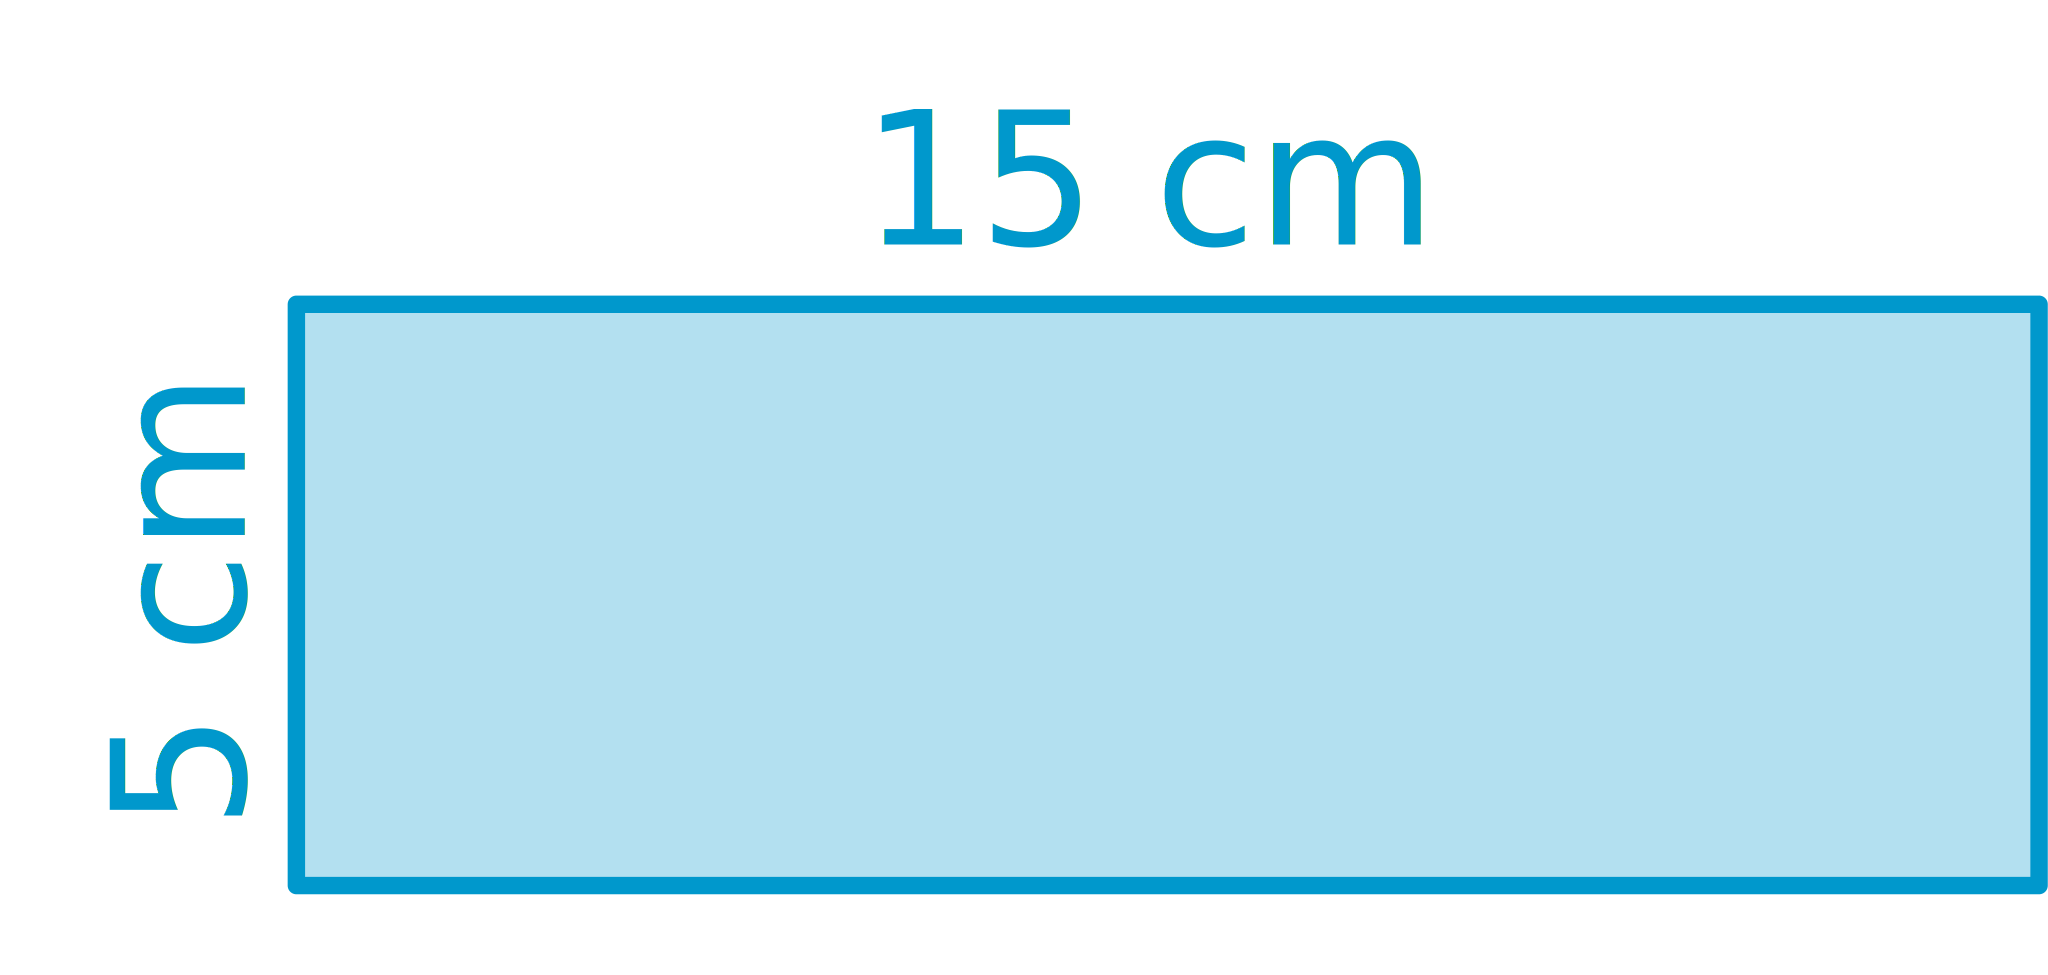
\includegraphics[width=3.8cm]{rect_cousin1} \end{center}
 \end{minipage} \hfill%
 \begin{minipage}[c]{0.48\linewidth}
 \begin{center} 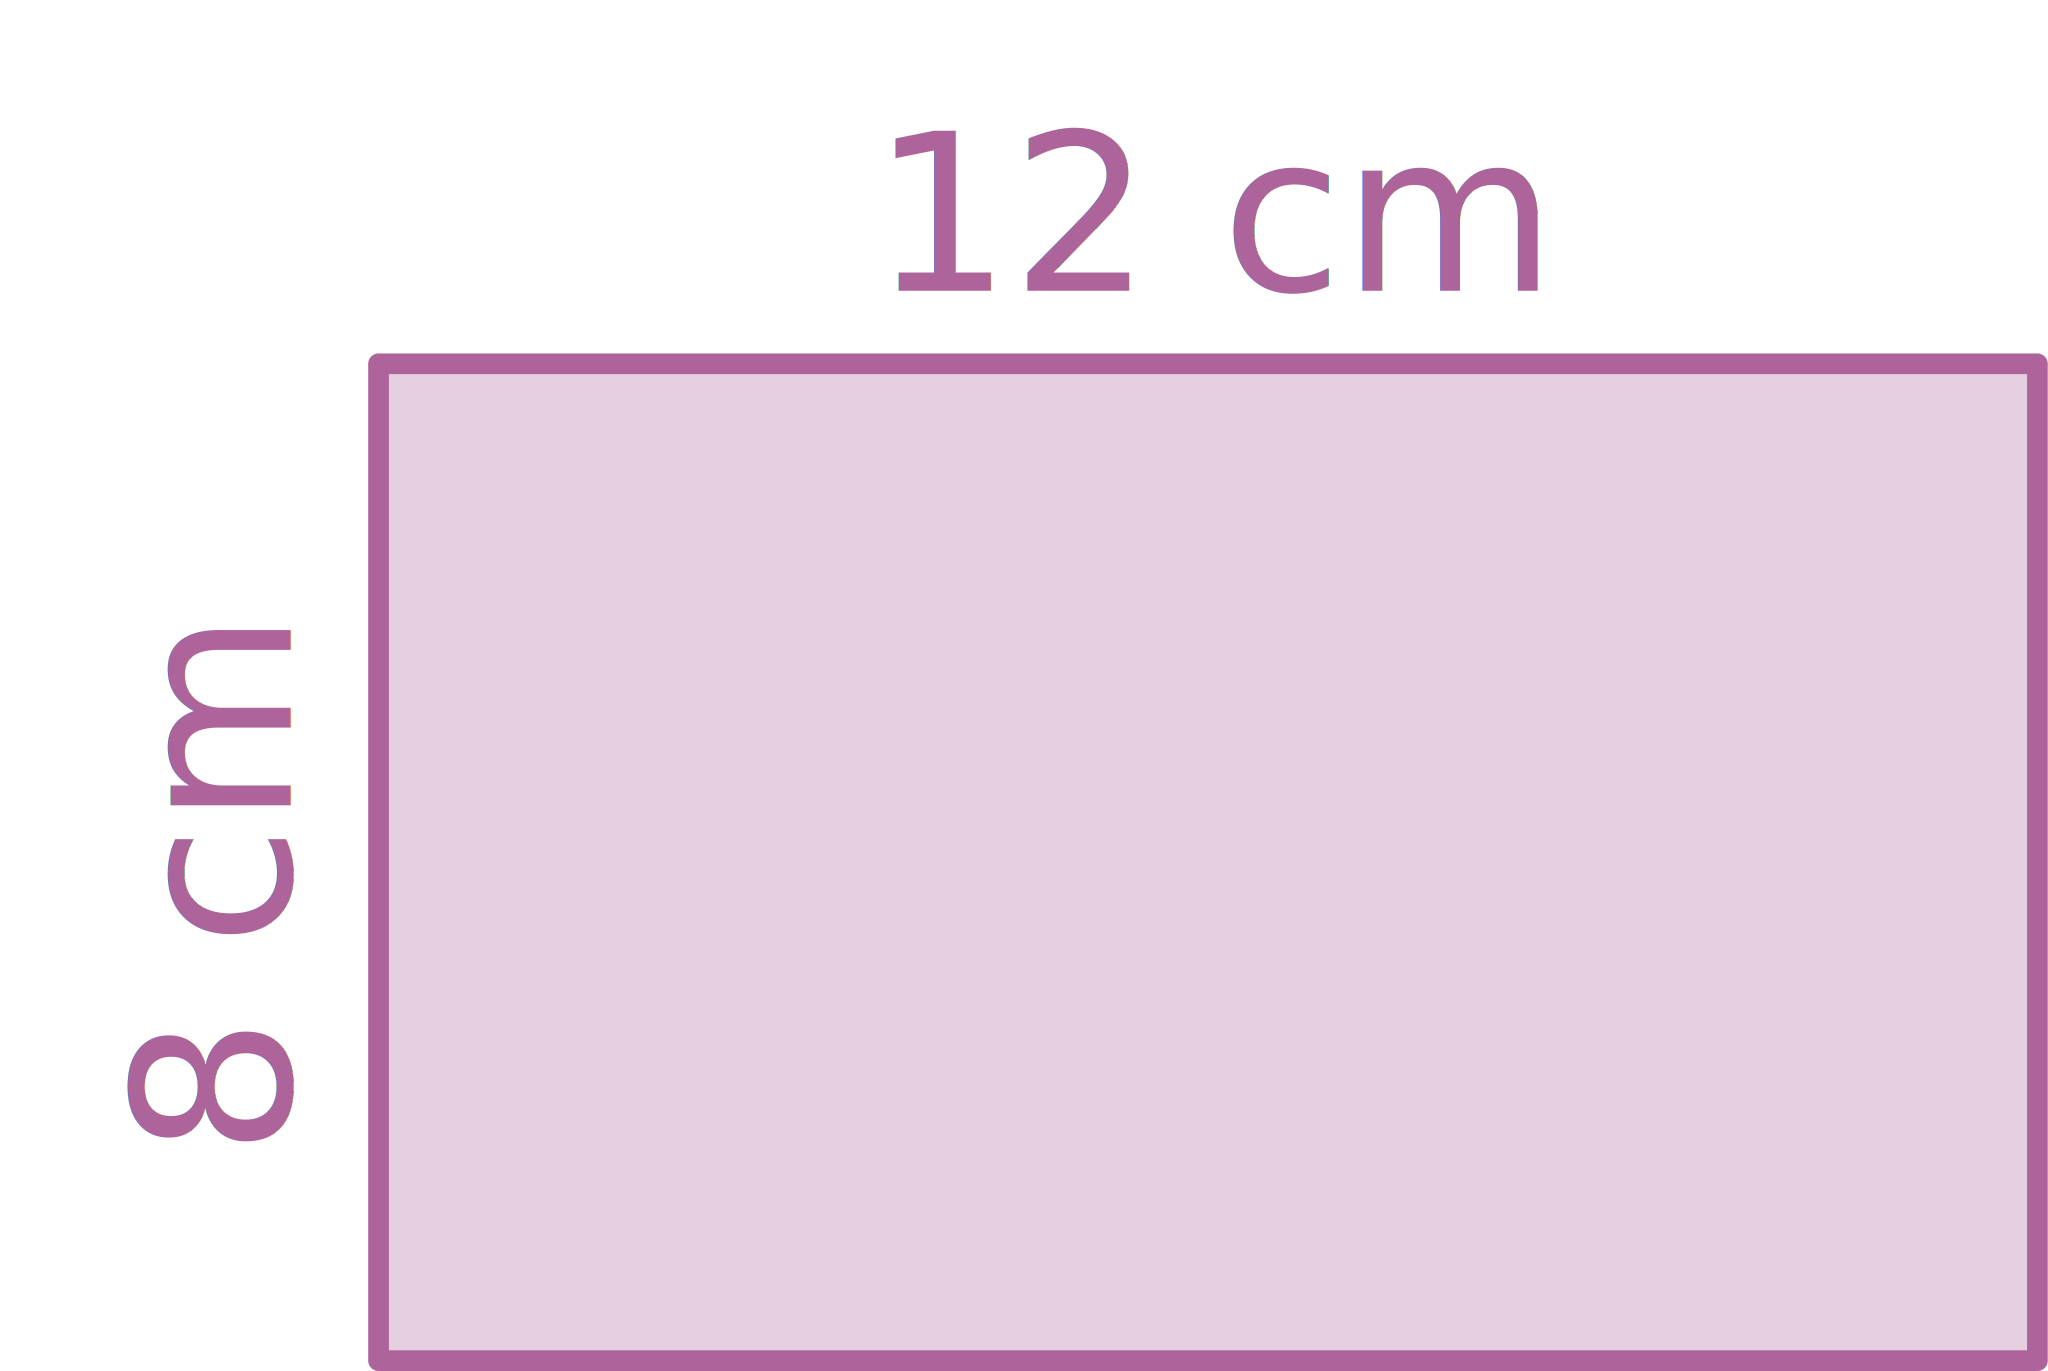
\includegraphics[width=3.3cm]{rect_cousin2} \end{center}
  \end{minipage}\\[0.5em]
Dans cette activité, on s'intéresse uniquement aux rectangles dont le périmètre est 40 cm.
\end{partie}


\begin{minipage}[c]{0.28\linewidth}
 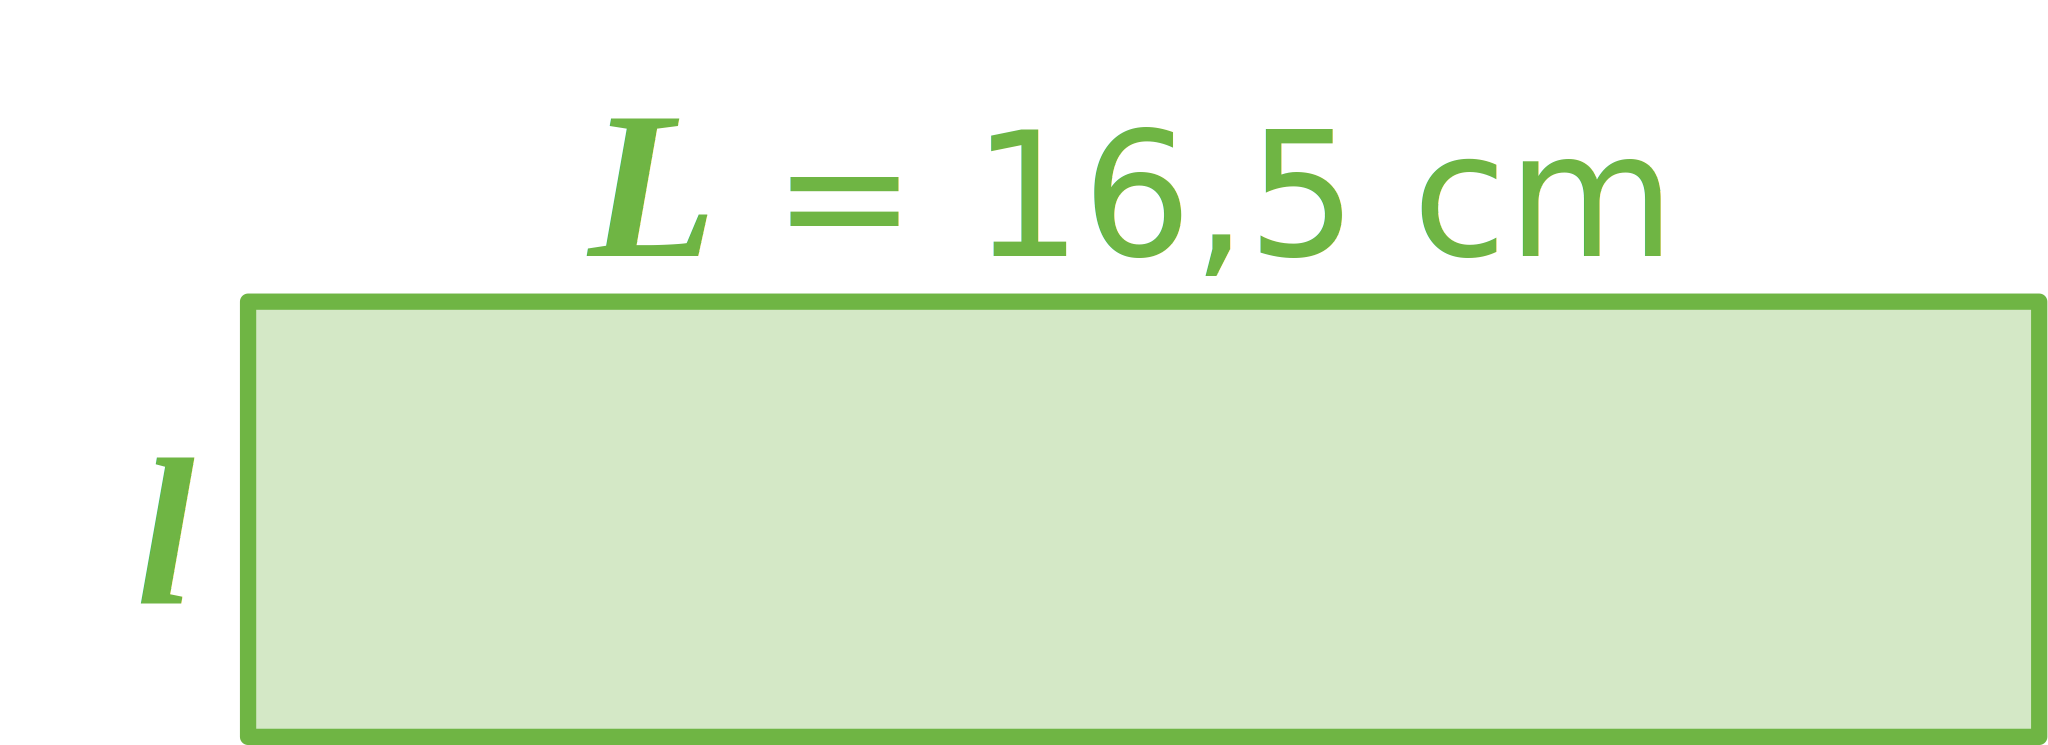
\includegraphics[width=4.3cm]{rect_cousin3}
 \end{minipage} \hfill%
 \begin{minipage}[c]{0.64\linewidth}
\vspace{1em}
\begin{partie}
Un 3\up{e} rectangle a pour longueur $\emph{\textbf{\textcolor{H1}{L}}} = 16,5\,\text{cm}$. Calcule sa largeur $\emph{\textbf{\textcolor{H1}{l}}}$ puis son aire.
\end{partie}

\begin{partie}
Donne les mesures d'un 4\up{e} rectangle de même périmètre.
\end{partie}
  \end{minipage} \\

\begin{partie}
La longueur peut-elle valoir 8 cm ? Et 21 cm ? Justifie et donne les valeurs possibles pour la longueur.
\end{partie}

\begin{partie}
Écris une expression qui permet de calculer la largeur $\emph{\textbf{\textcolor{H1}{l}}}$ en fonction de la longueur $\emph{\textbf{\textcolor{H1}{L}}}$.
\end{partie}

\begin{partie}
En voulant exprimer l'aire du rectangle en fonction de sa longueur $L$, des élèves ont donné les réponses suivantes :
\begin{center}
 \begin{tabularx}{1.1\linewidth}{X|X|X}
  Gaël : $A = L \cdot 20 - L$ & Hamid : $A = L \cdot (20 - L)$ & Karen : $A = 20\,L - L^2$ \\
  Inès : $A = 2 \cdot L + 2 \cdot (20 - L)$ & José : $A = L \cdot 20 - 2 \cdot L$ & Liam: $A = L^2 - 20 \cdot L$ \\
  \end{tabularx}   
 \end{center}
 \vspace{0.3cm}
Parmi ces expressions, lesquelles sont fausses ? Y a-t-il plusieurs bonnes réponses ? Justifie.
\end{partie}

\begin{partie}
Calcule l'aire de ces rectangles pour toutes les valeurs entières de $L$ possibles. Pour quelle valeur de $L$ l'aire semble-t-elle la plus grande ?
\end{partie}

\end{activite}


\cours
%\section{Une section}

% remarque : pour qu'un mot se retrouve dans le lexique : \MotDefinition{asymptote horizontale}{} 

\begin{aconnaitre}
Pour \MotDefinition{alléger l'écriture d'une expression littérale}{}, on peut supprimer le signe de multiplication "$\cdot$" devant une lettre ou une parenthèse.
\end{aconnaitre}

\begin{aconnaitre}
\begin{minipage}[t]{0.38\linewidth}
Pour tout nombre $a$, on peut écrire : 
 \end{minipage} \hfill%
\begin{minipage}[t]{0.58\linewidth}
\textcolor{H1}{$\pmb{a \cdot a = a^2}$} \hspace{1em} (qui se lit  « $a$ au carré ») \\[0.5em]
\textcolor{H1}{$\pmb{a \cdot a \cdot a = a^3}$} \hspace{1em} (qui se lit « $a$ au cube »).
 \end{minipage} \\
\end{aconnaitre}

\begin{methode*1}[Écrire une expression en respectant les conventions]

\begin{remarque}
On ne peut pas supprimer le signe "$\cdot$" entre deux nombres.
\end{remarque}
 
\begin{exemple*1}
Supprime les signes "$\cdot$", lorsque c'est possible, dans l'expression suivante : $A = 5 \cdot x + 7 \cdot (3 \cdot x + 2 \cdot 4)$.
\begin{center}
 \begin{tabular}{lcl}
$A = 5\,\textcolor{H1}{\cdot}\,x + 7\,\textcolor{H1}{\cdot}\,(3\,\textcolor{H1}{\cdot}\,x + 2\,\textcolor{H1}{\cdot}\,4)$ & $\longrightarrow$ & On repère tous les signes "\textcolor{H1}{$\cdot$}" de l'expression. \\ %dark green and bolt
$A = 5x + 7(3x + 2 \cdot 4)$ & $\longrightarrow$ & On supprime les signes "\textcolor{H1}{$\cdot$}" devant une lettre \\ %dark green and bolt
& &  ou une parenthèse.
  \end{tabular}
 \end{center}
\end{exemple*1}

\exercice  
Simplifie les expressions en supprimant le signe "$\cdot$" lorsque c'est possible :\\[1em]
$B = b \cdot a =$ \ldots \ldots;\\[1em]
$C = 5 \cdot x \cdot x \cdot x =$ \ldots \ldots \ldots \ldots;\\[1em]
$D = (3,7 \cdot y - 1,5 \cdot z + 0,4 \cdot 3,5) \cdot 9 =$ \ldots \ldots \ldots \ldots \ldots \ldots \ldots \ldots.
%\correction

\exercice  
Replace les signes "$\cdot$" dans chacune des expressions suivantes :\\[1em]
$E = 12\,a\,c + 35\,a\,b - 40\,b\,c$ \dotfill;\\[1em]
$F = 1,2\,a\,b\,c$ \dotfill;\\[1em]
$G = 5,6\,(x^2 - 2,5\,y + 32)$ \dotfill.
%\correction

\end{methode*1}
 
 %%%%%%%%%%%%%%%%%%%%%%%%%%%%%%%%%%%%%%%%%%%%%%%%%%%%%%%%%%%%%%%%%%%%%%%%
 %%%%%%%%%%%%%%%%%%%%%%%%%%%%%%%%%%%
%%%%%%%%%%%%%%%%%%%%%%%%%%%%%%%%%%%
%MiseEnPage
%%%%%%%%%%%%%%%%%%%%%%%%%%%%%%%%%%%
\newpage
%%%%%%%%%%%%%%%%%%%%%%%%%%%%%%%%%%%
%%%%%%%%%%%%%%%%%%%%%%%%%%%%%%%%%%%
 
 
\begin{aconnaitre}
Pour \MotDefinition{calculer une expression littérale pour une certaine valeur des lettres}{}, il suffit de remplacer les lettres par ces valeurs.
\end{aconnaitre}

\begin{methode*1}[Remplacer des lettres par des nombres]
 
\begin{exemple*1}
Calcule l'expression $A = 5x(x + 2)$ pour $x = 3$ :
\begin{center}
 \begin{tabular}{lcl}
$A = 5 \cdot x \cdot (x + 2)$ & $\longrightarrow$ & On replace les signes "$\cdot$" dans l'expression A. \\
$A = 5 \cdot \textcolor{H1}{\pmb{3}} \cdot (\textcolor{H1}{\pmb{3}} + 2)$ & $\longrightarrow$ & On remplace la lettre $x$ par sa valeur \textcolor{H1}{3}. \\ %dark green and bolt
$A = 15 \cdot 5$ & $\longrightarrow$ &  On effectue les calculs. \\
$A= 75$ & &
  \end{tabular}
 \end{center}
\end{exemple*1}

\exercice  
Calcule les expressions suivantes pour $x = 2$ puis pour $x = 6$ :\\[1em]
$B = 3\,x(x + 5)$ \dotfill;\\

\dotfill \\[1em]
$C = 7x - x^2$ \dotfill;\\

\dotfill \\[1em]
$D = x^3 + 3x^2 - x$\dotfill.\\

\dotfill
%\correction

\exercice  
Calcule les expressions pour $a = 3$ et $b = 5$ :\\[1em]     
$E = 4a + 5b - 56$ \dotfill;\\

\dotfill \\[1em]
$F = a^3 + b^2 + 7ab$ \dotfill;\\

\dotfill \\[1em]
$G = 2(5a + 3b + 1)$ \dotfill;\\.

\dotfill \\[1em]
%\correction

\end{methode*1}


\exercicesbase
\begin{colonne*exercice}

\serie{Simplifier une expression littérale}

\begin{exercice}
Recopie les expressions suivantes en supprimant le signe "$\cdot$" s'il est inutile :
\begin{colitemize}{2}
 \item $A = 9 \cdot n$ ;
 \item $B = x \cdot 3$ ;
 \item $C = 12 \cdot (7 - 3)$ ;
 \item $D = 4 \cdot (3,2 + 6)$ ;
 \item $E = n \cdot x$ ;
 \item $F = 2 \cdot 6$ ;
 \item $G = (3 + 6) \cdot (7 - 1)$ ;
 \item $H = 16 \cdot 3,5 \cdot R$.
 \end{colitemize}
\end{exercice}


\begin{exercice}
Recopie les expressions suivantes en ajoutant le signe "$\cdot$" lorsqu'il est sous-entendu :
\begin{colitemize}{2}
 \item $A = 3x + 2$ ;
 \item $B = ab - 4$ ;
 \item $C = 5(2x - 7)$ ;
 \item $D = 2a(2 + 8)$ ;
 \item $E = 3a - 5b$ ;
 \item $F = ab + 3 \cdot 7a$ ;
 \item $G = b - a + 7(3x + 7)$ ;
 \item $H = a + a - 7b + 1$.
 \end{colitemize}
\end{exercice}


\begin{exercice}
Écris les expressions suivantes le plus simplement possible :
\begin{colitemize}{2}
 \item $A = 3 \cdot a \cdot b$ ; 
 \item $B = 3 \cdot a - 4 \cdot b$ ; 
 \item $C = 8 \cdot a \cdot b \cdot 2$ ;
 \item $D = 3 \cdot (2 \cdot a + b) \cdot 5$ ;
 \item $E = 2 \cdot 3 + 7 - 1$ ;
 \item $F = 2 + 5 + 3 \cdot b$ ; 
 \item $G = (2,5 - 1) \cdot a \cdot b$ ; 
 \item $H = 2 \cdot 3 \cdot a \cdot (b \cdot c)$.
 \end{colitemize}
\end{exercice}


\begin{exercice}
Écris les expressions suivantes le plus simplement possible en utilisant les notations "au carré" et "au cube" si nécessaire :
\begin{colitemize}{2}
 \item $A = 1 \cdot a + a \cdot a$ ;
 \item $B = a \cdot a \cdot a - 0 \cdot b$ ;
 \item $C = 6 \cdot a \cdot a - a$ ; 
 \item $D = 2 \cdot a \cdot 3 \cdot a$ ; 
 \item $E = a \cdot a \cdot b \cdot 3$ ;
 \item $F = 1 \cdot a \cdot a \cdot b \cdot 0$ ;
 \item $G = a \cdot 2 \cdot b \cdot a \cdot b$ ;
 \item $H = (a + b) \cdot (a + b)$.
 \end{colitemize}
Aire d'un carré de côté $c$ : $c \cdot c = \ldots$
\end{exercice}


\begin{exercice}
Traduis par une expression littérale les phrases suivantes :
\begin{enumerate}
 \item La somme de $x$ et de 13 ;
 \item Le double de $x$ ;
 \item La différence de $x$ et de 7 ;
 \item Le tiers de $x$ ;
 \item Le triple de la somme de 2 et de $x$ ;
 \item Le tiers de la différence entre 16 et $x$.
 \end{enumerate}
\end{exercice}


\begin{exercice}
Calcule les expressions suivantes pour les valeurs de $x$ et de $y$ indiquées :
\begin{colitemize}{2}
 \item $A = 4 x + 3$ ;
 \item $B	= 3 x^2$ ;
 \item $C	= x y - x - y + 4$ ;
 \item $D	= x^2 + 2xy + y^2$ ;
 \item $E	= x^2 + y^2$ ;
 \item $F	= x^2 y$.
 \end{colitemize}
 \begin{enumerate}
  \item Pour $x = 2$ et $y = 3$ ;
  \item Pour $x = 3$ et $y = x$.
  \end{enumerate}
\end{exercice}

%%%%%%%%%%%%%%%%%%%%%%%%%%%%%%%%%%%%%%%%%%%%%%%%%%%%%%%%%%%%%%%%%%%%%%%%%

\serie{Produire une expression littérale}

\begin{exercice}[Périmètres]
\begin{enumerate}
 \item Exprime le périmètre des figures ci-dessous en fonction de $a$ et de $b$ sachant qu'un trait bleu mesure $a$ cm, un trait rose mesure $2a$ cm et un trait vert mesure $b$ cm :
 
\begin{minipage}[c]{0.48\linewidth}
 \begin{center} 
\includegraphics[width=2.5cm]{perimetre1} \end{center}
 \end{minipage} \hfill%
 \begin{minipage}[c]{0.48\linewidth}
  \begin{center} 
\includegraphics[width=2.9cm]{perimetre2} \end{center} 
  \end{minipage} \\
 \item Calcule ensuite ces deux périmètres pour $a = 1,3$ et $b = 4$.
 \end{enumerate}
\end{exercice}


\begin{exercice}[Aire en fonction de $x$]
\begin{minipage}[c]{0.48\linewidth}
 \begin{enumerate}
  \item Calcule l'aire de la partie coloriée en fonction de $x$.
  \item Combien vaut cette aire si $x = 14,7 \text{m}$ ?
  \end{enumerate}
 \end{minipage} \hfill%
 \begin{minipage}[c]{0.48\linewidth}
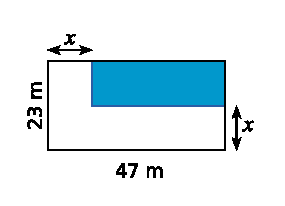
\includegraphics[width=4.1cm]{aire_fx}
  \end{minipage} \\
\end{exercice}


\begin{exercice}
Pour son téléphone portable, Grégoire paye : 12 CHF d'abonnement, $a$ CHF par SMS envoyé et 40 centimes par minute de communication. 
\begin{enumerate}
 \item Écris une expression permettant de calculer sa dépense sachant que ce mois-ci, Grégoire a envoyé 30 SMS et a utilisé $m$ minutes de communications.
 \item Quelle est cette dépense si $a = 0,8$ et $m = 150$ ?
 \end{enumerate}
\end{exercice}


\begin{exercice}
Sandrine a construit un triangle tel que la longueur d'un petit côté vaut la moitié de celle du grand et la longueur du moyen vaut les trois quarts de celle du grand.
\begin{enumerate}
 \item Écris une expression permettant de calculer le périmètre du triangle en fonction de la longueur $L$ du plus grand des côtés ;
 \item Détermine le périmètre si $L$ vaut 7 cm.
 \end{enumerate}
\end{exercice}


%%%%%%%%%%%%%%%%%%%%%%%%%%%%%%%%%%%
%%%%%%%%%%%%%%%%%%%%%%%%%%%%%%%%%%%
%MiseEnPage
%%%%%%%%%%%%%%%%%%%%%%%%%%%%%%%%%%%
\newpage
%%%%%%%%%%%%%%%%%%%%%%%%%%%%%%%%%%%
%%%%%%%%%%%%%%%%%%%%%%%%%%%%%%%%%%%

\begin{exercice}
Marc a rentré trois nombres en mémoire dans sa machine à calculer. Pour cela, il a utilisé les lettres $a$, $b$ et $c$. Il veut maintenant calculer les expressions suivantes :
\begin{itemize}
 \item $S = 2a - 3b + 7c + 5$ ;
 \item $T = 7ab + 4c - 8$.
 \end{itemize}
Calcule ces expressions pour $a = 12$, $b = 5$ et $c = 7$. Vérifie les résultats obtenus à l'aide de ta calculatrice.
\end{exercice}


\begin{exercice}
Exprime en fonction de $x$ et $y$ les périmètres du carré et du rectangle suivants :
\begin{center} 
\includegraphics[width=4.3cm]{rectangles_xy} \end{center} 
Pour les valeurs de $x$ et de $y$ suivantes, le périmètre du carré est-il supérieur à celui du rectangle ?
\begin{colenumerate}{2}
 \item $x = 2$ et $y = 1$ ; 
 \item $x = 3$ et $y = 1$ ; 
 \item $x = 6$ et $y = 3$ ; 
 \item $x = 10$ et $y = 7$.
 \end{colenumerate}
\end{exercice}


\begin{exercice}[La grande bleue]
\begin{center} 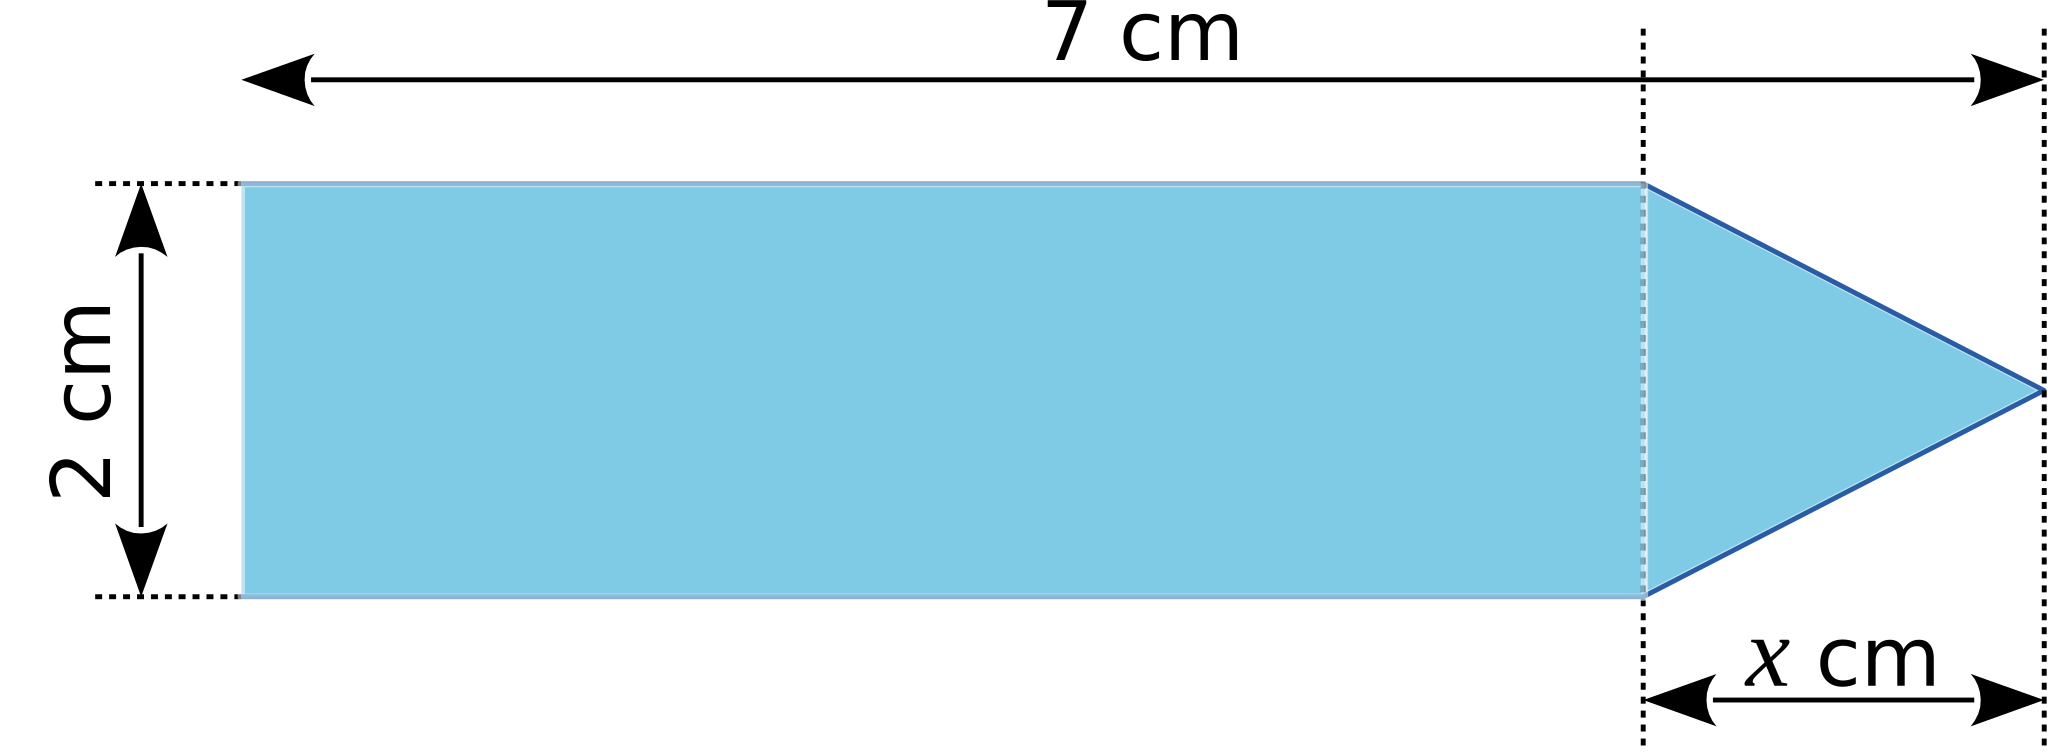
\includegraphics[width=8.1cm]{grande_bleue} \end{center}
\begin{enumerate}
 \item Exprime l'aire de la surface bleue en fonction de $x$ ;
 \item Calcule cette aire pour $x = 3 cm$.
 \end{enumerate}
\end{exercice}


\begin{exercice}
Marie dit qu'en ajoutant deux nombres impairs, on obtient toujours un nombre impair :
\begin{enumerate}
 \item Prouve-lui qu'elle a tort à l'aide d'un contre-exemple ;
 \item En utilisant la variable $n$, écris une expression désignant un nombre pair puis une autre désignant un nombre impair ; \label{CalcLit_entrain1}
 \item Utilise la question \ref{CalcLit_entrain1} pour démontrer à Marie que la somme de deux nombres impairs n'est jamais impaire.
 \end{enumerate}
\end{exercice}


\begin{exercice}
Vanessa a acheté un cahier à 2 CHF et trois classeurs à $x$ CHF :
\begin{enumerate}
 \item Exprime le prix total qu'elle a payé en fonction de $x$ ;
 \item Elle a payé 23 CHF en tout. Retrouve le prix d'un classeur.
 \end{enumerate}
\end{exercice}


\begin{exercice}[Un carré qui grandit]
Soit $ABCD$ un carré de 5 cm de côté :
\begin{enumerate}
 \item Calcule le périmètre et l'aire de $ABCD$.
 \end{enumerate}
On augmente son côté de $k$ cm. Exprime, en fonction de $k$ :
\begin{enumerate}
\setcounter{enumi}{1}
 \item La longueur $L$ de ce nouveau côté ;
 \item Le nouveau périmètre $P$ de ce carré ;
 \item La nouvelle aire $S$ de ce carré ;
 \item L'augmentation $A_p$ du périmètre ;
 \item L'augmentation $A_s$ de l'aire.
 \end{enumerate}
\end{exercice}

\end{colonne*exercice}


\exercicesappr
\begin{colonne*exercice}
\begin{exercice}[Tracé d'un U dans une feuille]
 \begin{minipage}[c]{0.58\linewidth}
 En cours d'Arts Plastiques, le professeur distribue aux élèves des feuilles carrées de 15 cm de côté. Il leur demande de découper un rectangle de largeur 5 cm pour former la lettre U. 
  \end{minipage} \hfill%
  \begin{minipage}[c]{0.38\linewidth}
  
\includegraphics[width=3.1cm]{U_rose}
  \end{minipage} \\
\begin{enumerate}
 \item Marine découpe un rectangle de longueur 8 cm (et de largeur 5 cm). Calcule le périmètre du U de Marine.
 \item Ses amies Alison et Laura ont découpé des rectangles de largeur 5 cm mais de longueurs différentes : celui d'Alison a une longueur de 6,3 cm alors que celui de Laura a une longueur de 9,6 cm. Calcule les périmètres des U d'Alison et de Laura. Quelle partie du calcul est la même pour tous les U ? 
 \item Après tous ces calculs, Kévin remarque que si $L$ désigne la longueur du rectangle en centimètres et $P$ le périmètre du U en centimètres, alors $P = 60 + 2L$ . Calcule $P$ lorsque $L = 7,5 \text{cm}$ et lorsque $L = 10 \text{cm}$.
 \item Priscilla dit : « On peut encore simplifier : $60 + 2 = 62$ donc $P = 62 L$ ». Utilise l'expression proposée par Priscilla pour calculer $P$ lorsque $L = 10 \text{cm}$. Que penses-tu de sa proposition ? Pourquoi ?
 \end{enumerate}
\end{exercice}


\begin{exercice}[Construction d'un escalier]

\vspace{1em}
 \begin{minipage}[c]{0.68\linewidth}
Clémence a fabriqué un escalier de quatre marches à l'aide de briques bleues toutes identiques d'un jeu de construction. Martin a ajouté des briques jaunes (toutes identiques) afin de former le même escalier « à l'envers » au dessus.
  \end{minipage} \hfill%
  \begin{minipage}[c]{0.28\linewidth}
  
\includegraphics[width=2.8cm]{escalier_duplo}
  \end{minipage} \\
\begin{enumerate}
 \item Quel est le nombre de briques bleues utilisées ? Écris-le sous la forme d'une somme.
 \item Clémence rajoute des briques bleues pour obtenir une cinquième marche à son escalier. À son tour, Martin rajoute autant de briques jaunes pour avoir le même escalier « à l'envers ».
 \begin{itemize}
  \item Réalise un dessin représentant les deux escaliers. Ils forment un rectangle.
  \item Quel est alors le nombre total de briques utilisées ? Écris-le sous la forme d'un produit.
  \item Déduis-en la valeur de $1 + 2 + 3 + 4 + 5$.
  \end{itemize}
  \item Sans faire de dessin, donne le nombre total de briques qu'il faudrait si on rajoutait une sixième marche à chacun des deux escaliers. Quel serait alors le nombre de briques bleues ? Déduis-en la valeur de $1 + 2 + 3 + 4 + 5 + 6$.
  \item On appelle $n$ le nombre de marches d'un escalier :
  \begin{itemize}
   \item Écris une expression qui indique le nombre total de briques nécessaires à la construction de deux escaliers de $n$ marches.
   \item Et pour un seul escalier ?
   \item Quelle égalité peut-on alors écrire ?
   \end{itemize}
  \item Combien de briques faut-il pour construire un escalier de 30 marches ? Et pour un escalier de 300 marches ?
 \end{enumerate}
\end{exercice}


\begin{exercice}[La pyramide de Gelo]
\vspace{1em}
 \begin{minipage}[c]{0.68\linewidth}
 Maurice a construit une pyramide de briques Gelo comme ci-dessous. Il y a une brique au premier étage, 4 briques au deuxième étage, 9 briques au troisième étage \ldots
  \end{minipage} \hfill%
  \begin{minipage}[c]{0.28\linewidth}
  
\includegraphics[width=3cm]{gelo}
  \end{minipage} \\
\begin{enumerate}
 \item Combien y a-t-il de briques au $4^\text{e}$ étage ? Au $20\text{e}$ étage ? Au $n^\text{e}$ étage ?
 \item Combien y a-t-il de briques au total lorsque la pyramide compte un étage ? Deux étages ? Trois étages ? Quatre étages ? \label{CalcLit_approf}
 \end{enumerate}
Maurice veut savoir combien de briques seront nécessaires pour construire une pyramide à vingt étages. Ne voulant pas faire un gros calcul, il cherche sur internet une formule lui donnant le résultat. Il a trouvé les trois expressions suivantes où $n$ représente le nombre d'étages :
\begin{center} $A = - 6n + 7$ \end{center}
\begin{center} $B = \dfrac{5n^2 - 7n + 4}{2}$ \qquad $C = \dfrac{n(n + 1)(2n +1)}{6}$ \end{center}
Maurice veut alors vérifier la véracité de ces informations.
\begin{enumerate}
\setcounter{enumi}{2}
 \item En testant chacune des formules avec les valeurs trouvées à la question \ref{CalcLit_approf}, quelles sont les formules que l'on peut éliminer d'office ?
 \item Maurice demande à son professeur si la formule non éliminée est exacte. Il lui répond par l'affirmative. Combien de briques sont nécessaires pour construire cette pyramide à vingt étages ?
 \end{enumerate}
\end{exercice}



\end{colonne*exercice}

\connaissances

\QCMautoevaluation{Pour chaque question, plusieurs réponses sont
  proposées.  Déterminer celles qui sont correctes.}

\begin{QCM}
  \begin{GroupeQCM}
    \begin{exercice}
      $5 \cdot x + 2 \cdot y =$
      \begin{ChoixQCM}{4}
      \item $10xy$
      \item $5x + 2y$
      \item $7xy$
      \item $7x + y$
      \end{ChoixQCM}
\begin{corrige}
     \reponseQCM{b}
   \end{corrige}
    \end{exercice}
    
    
    \begin{exercice}
      $3x^2y$ est le résultat de \ldots
      \begin{ChoixQCM}{4}
      \item $6x \cdot y$
      \item $3x \cdot y$
      \item $3x \cdot xy$
      \item $y \cdot 3x^2$
      \end{ChoixQCM}
\begin{corrige}
     \reponseQCM{cd}
   \end{corrige}
    \end{exercice}
    
    
    \begin{exercice}
      Soit $A = 5x$. Si on remplace $x$ par 5, alors $A = \ldots$
      \begin{ChoixQCM}{4}
      \item 55
      \item 25
      \item 10
      \item $5 \cdot 2$
      \end{ChoixQCM}
\begin{corrige}
     \reponseQCM{b}
   \end{corrige}
    \end{exercice}
    
    
    \begin{exercice}
      Quels sont les nombres qui vérifient l'inégalité \hspace{1em} $t - 5 < 2t + 3$ ?
      \begin{ChoixQCM}{4}
      \item 0
      \item 2
      \item $- 9$
      \item 10
      \end{ChoixQCM}
\begin{corrige}
     \reponseQCM{abd}
   \end{corrige}
    \end{exercice}


\end{GroupeQCM}
\end{QCM}

  


\TravauxPratiques % pour nous "travailler en groupe"

\begin{TP}[Boîte noire \ldots]

\partie{Pour bien démarrer \ldots}
\begin{enumerate}
 \item Voici un programme de calcul : \label{CalcLit_TP1}
 \begin{itemize}
  \item \textbf{\textcolor{C2}{Choisir un nombre}} ;
  \item \textbf{\textcolor{C2}{Multiplier ce nombre par 3}} ;
  \item \textbf{\textcolor{C2}{Ajouter 4 au résultat précédent}}.
  \end{itemize}
 Appliquez ce programme pour les nombres : 3 ;  5 et 2,5.
 \item On considère l'expression : $A = 3 x + 4$. Calculez $A$ pour $x = 5$ puis pour $x = 2,5$. Que remarquez-vous ? Expliquez pourquoi. \label{CalcLit_TP2}
 \item Quel programme de calcul correspond à l'expression $B = 7 x - 3$ ?
 \item Essayez de construire un programme de calcul permettant d'obtenir 5 quand on choisit 2 pour nombre de départ. Y a-t-il une seule solution selon vous ?
 \item Achille a écrit un programme de calcul sur son cahier mais il l'a oublié chez lui. Il avait noté sur une feuille à part le tableau suivant : \label{CalcLit_TP3}
 \vspace{0.3cm}
 \begin{center}
  \renewcommand*\tabularxcolumn[1]{>{\centering\arraybackslash}m{#1}}
  \begin{Ctableau}{0.8\linewidth}{4}{c}
   \hline
Nombre de départ & 2 & 4 & 17 \\\hline
Résultat du programme & 9 & 11 & 24 \\\hline
   \end{Ctableau}
 \end{center}
 \vspace{0.3cm}
 À partir de ce tableau, pouvez-vous retrouver un programme de calcul qui conviendrait ?
 \item À l'aide de ce programme, recopiez le tableau précédent puis complétez-le avec trois nouveaux nombres de départ : 5,5 ; 7 et 3,1.
 \item Donnez l'expression avec la lettre $x$ qui correspond à ce programme.
 \item Voici un autre tableau de valeurs :
 \vspace{0.3cm}
 \begin{center}
  \renewcommand*\tabularxcolumn[1]{>{\centering\arraybackslash}m{#1}}
  \begin{Ctableau}{0.8\linewidth}{4}{c}
   \hline
Nombre de départ & 2 & 10 & 1,5 \\\hline
Résultat du programme & 5 & 21 & 4 \\\hline
   \end{Ctableau}
 \end{center}
 \vspace{0.3cm}
Leïla dit que l'expression $C = 3 x - 1$ pourrait parfaitement convenir à un tel tableau. Expliquez pourquoi elle se trompe.
 \item Trouvez un programme de calcul et l'expression associée qui conviendrait pour ce nouveau tableau.
 \end{enumerate}
        
\partie{Boîte noire}

Quand on rentre un nombre dans une boîte noire, elle exécute un programme de calcul pour fournir un résultat. \\[0.5em]
L'objectif de cette partie est de construire des boîtes noires puis d'essayer de démasquer les boîtes noires d'un autre groupe. \\[0.5em]
\begin{enumerate}
\setcounter{enumi}{9}
 \item Vous allez construire deux boîtes noires : une facile et une difficile. La construction de ces boîtes doit rester secrète pour garder le mystère. Pour chacune de ces deux boîtes, il faut :
 \vspace{0.3cm}
 \begin{itemize}
  \item Trouver un programme de calcul, comme à la question \ref{CalcLit_TP1} (les nombres utilisés doivent être des entiers plus petits que 10) ;
  \item Trouver l'expression qui correspond, comme à la question \ref{CalcLit_TP2} ; 
  \item Faire un tableau comme à la question \ref{CalcLit_TP3}, avec trois valeurs et les résultats obtenus.
  \end{itemize}
 \vspace{0.3cm}
Pour la boîte facile, le programme ne peut comporter qu'une seule fois la lettre $x$. \\[0.5em]
Pour la boîte difficile, le programme ne peut comporter qu'un seul terme avec  $x^2$.
 \vspace{0.3cm}
 \item Une fois que vous avez construit vos boîtes, écrivez les deux tableaux de valeurs sur une même feuille. Vérifiez bien que vos tableaux sont corrects ! Échangez cette feuille avec la feuille d'un autre groupe.
 \item Quand un groupe pense avoir réussi à décoder une boîte noire, il peut s'en assurer en demandant au groupe qui l'a créée le résultat que donnerait la boîte noire pour la valeur de leur choix. Le défi est relevé quand un groupe est capable d'écrire sur une feuille le programme et l'expression correspondante pour chacune des boîtes noires.
 \end{enumerate}
\underline{Attention} : Si un groupe s'est trompé dans ses calculs pour réaliser le tableau alors c'est ce groupe qui aura perdu le défi !

\end{TP}



\pagebreak

\recreation
\begin{enigme}[Les yeux dans l'œil !]

\begin{minipage}[c]{0.48\linewidth}
Sur la planète Volcoudoeil, il y a deux populations : les Kachmoipalavu qui n'ont qu'un oeil et les Jeupeutouzieuter qui en ont trois. \\[0.5em]
Lors de ma dernière visite sur cette planète, une photo a été prise. J'y figurais avec mes meilleurs amis, issus de ces deux populations. Bref, une photo de 13 personnes et 24 yeux dont les deux miens. \\[0.5em]
Combien de Kachmoipalavu y avait-il sur cette photo ?
 \end{minipage} \hfill%
 \begin{minipage}[c]{0.48\linewidth}
  \includegraphics[width=8.1cm]{mono_oeil}
  \end{minipage} \\

\end{enigme} 



